\section{Programmation système : Système de fichiers}
\subsection{Contexte}
La	carte ODROID-XU3	Lite	est	équipé	d’un	petit	ventilateur	afin	d’évacuer	la	chaleur	produite	par	
l’activité	du	microprocesseur.	La	vitesse	du	ventilateur	est	contrôlée par	un	PWM	(Pulser-Width	
Modulation),	dont	le	rapport	de	cycle	(duty)	dépendra	de	la	température	du	microprocesseur.	Le	
ventilateur	sera	régulé	sur	la	base	de	20kHz.		Sur	la	carte	ODROID-XU3	Lite	ce	PWM	peut	être	réalisé	
avec	la	porte	d’entrée/sortie	"gpb2\_0".
\subsection{Travail à réaliser}
Sur	le	site	moodle	vous	trouverez	une	petite	application	qui	contrôle	la	vitesse	du	ventilateur.	Ce	code	
n’a	pas	été	très	bien	programmé	et	utilise	le	100\%	d’un	cœur	du	processeur	(à	mesurer	avec	top).	
Concevez	une	application	permettant	de	gérer	la	vitesse	de	rotation	du	ventilateur	de	l’ODROID-XU3	
à	l’aide	des	trois	boutons	poussoir.
Quelques	indications	pour	la	réalisation de	l’application :
\begin{enumerate}
\item Au	démarrage	le	duty	cycle	du	ventilateur	sera	réglé	à	50\%
\item Utilisation	des	boutons	poussoir
\begin{enumerate}
\item « sw1 »	pour	augmenter	la	vitesse	du	ventilateur
\item « sw2 »	pour	remettre	la	vitesse	du	ventilateur	à	sa	valeur	initiale
\item « sw3 »	pour	diminuer	la	vitesse	du	ventilateur
\item une	pression	continue	exercée	sur	un	bouton	indiquera	une	auto	incrémentation	
ou	décrémentation	du	duty	cyle.
\end{enumerate}
\item Tous	les	changements	de	vitesse	du	ventilateur	seront	logger	avec	syslog	de	Linux.
\item Le	multiplexage	des	entrées/sorties	devra	être	utilisé.
\end{enumerate}

\subsection{Travail réalisé}
\subsubsection{Description}
Tous les points de la donnée ont été implémentés. La fréquence du ventilateur a été augmentée à 50 kHz, car à 20kHz le ventilateur émet un son strident très agaçant.\\Pour le point de l'auto incrémentation, la duty cycle est augmenté/diminué de 2\% chaque 40 us quand un bouton est maintenu appuyé. Si par hasard, on maintient appuyé deux boutons en même temps, le programme attend qu'un des deux soit relâché pour changer le duty cycle.\\En plus des points demandés, les LEDs de la carte d'extensions sont utilisées.
\begin{enumerate}
	\item LED1: S'allume et s'éteint en fonction de la pression sur le switch 1.
	\item LED2 : Clignote à la fréquence de la PWM. La vitesse est trop rapide pour la voir clignoter, on peut par contre observer un changement de luminosité entre un duty cycle proche de 0\% et un proche de 100\%.
	\item LED3 : S'allume et s'éteint en fonction de la pression sur le switch 3.\\
\end{enumerate} 

\textbf{Emplacement du code : } \textit{/FanControl}

\subsubsection{Configuration des GPIO}
Une des recherches à faire pour ce projet était de trouvé à quelle GPIO correspondait les boutons, les LEDs et le ventilateur.\\
Pour cela, la schématique de la carte d'extension a été utilisée.\\\\
Source : \url{http://dn.odroid.com/ODROID-XU/Expansion_Board/ExpansionBoard.pdf}\\\\
Si on prend comme exemple la LED D1, on trouve dans le schéma qu'elle correspond à la pin XE.INT23. Pour obtenir la GPIO correspondante, cette page a été très utile.\\\\
Source : \url{http://odroid.com/dokuwiki/doku.php?id=en:odroid-xu}\\\\
On apprend grâce à ce site que la pin XE.INT23 correspond au GPX2.7.\\
Pour trouver le numéro de GPIO correspondant, il suffit d'entrer les commandes suivantes sur la cible:
\begin{lstlisting}
# mount -t debugfs none /sys/kernel/debug                                       
# cat /sys/kernel/debug/gpio                                                    
...
GPIOs 16-23, platform/13400000.pinctrl, gpx1:                                   
gpio-17  (dwc3_id_gpio        ) in  hi                                         
gpio-19  (sysfs               ) out lo                                         
gpio-22  (sysfs               ) in  hi                                         
gpio-23  (scl                 ) out hi                                         

GPIOs 24-31, platform/13400000.pinctrl, gpx2:                                   
gpio-27  (red:activity        ) out lo                                         
gpio-28  (sysfs               ) out hi                                         
gpio-29  (sysfs               ) in  hi                                         
gpio-30  (sysfs               ) in  hi                                         
gpio-31  (sysfs               ) out lo                                         
...   
\end{lstlisting}
Ces commandes nous renseignent sur le numéro de GPIO. Si l'on reprend l'exemple de la LED D1, on va lire que le GPX2 correspond au numéro 24. Comme la LED est sur le GPX2.7, il faut encore rajouter l'offset. On obtient donc 24+7 = \textbf{31} comme numéro de GPIO pour la LED D1.\\
Pour configurer les entrées/sorties, le code pour atteindre la pwm fourni dans l'exemple a été repris. Pour les boutons ils suffit d'ajouter le flanc de détection pour l'interruption.
\subsubsection{Exécution du code}
Le code s'exécute dans l'espace utilisateur et non plus dans le noyau comme les exercices précédents. Le code doit être compilé sur l'hôte et lancé sur la cible (en mode nfs). L'application n'affiche rien directement dans la console, tout est dans le syslog.
\begin{lstlisting}
lmi@csel1:~/workspace/csel1/environment/fanCtrl$ make clean all
\end{lstlisting}
\begin{lstlisting}
# cd /usr/workspace/csel1/environment/fanCtrl/
# ./app_a  
\end{lstlisting}
\subsubsection{Syslog}
Une fois l'application lancée, on peut aller voir le \textit{syslog}. Le duty cycle du ventilateur y est affiché chaque fois qu'il change. Comme l'application est lancée depuis la connexion sérielle, il faut accéder à la cible par connexion ssh. Chaque pression sur un des boutons fera afficher une nouvelle ligne.\\
\begin{lstlisting}
lmi@csel1:~$ ssh root@192.168.0.11
# tail -f /var/log/messages
Jan  1 00:06:37 odroidxu3 local1.notice fan control[1625]: duty :64
Jan  1 00:06:37 odroidxu3 local1.notice fan control[1625]: duty :66
Jan  1 00:06:37 odroidxu3 local1.notice fan control[1625]: duty :68
Jan  1 00:06:37 odroidxu3 local1.notice fan control[1625]: duty :70
Jan  1 00:06:37 odroidxu3 local1.notice fan control[1625]: duty :72
...
\end{lstlisting}
\subsubsection{Mesure de performance}
La commande \textit{top} permet de mesurer les performances de l'application. Le code fourni en exemple utilise 100\% d'un cœur du processeur.
\begin{figure}[H]
	\begin{center}
		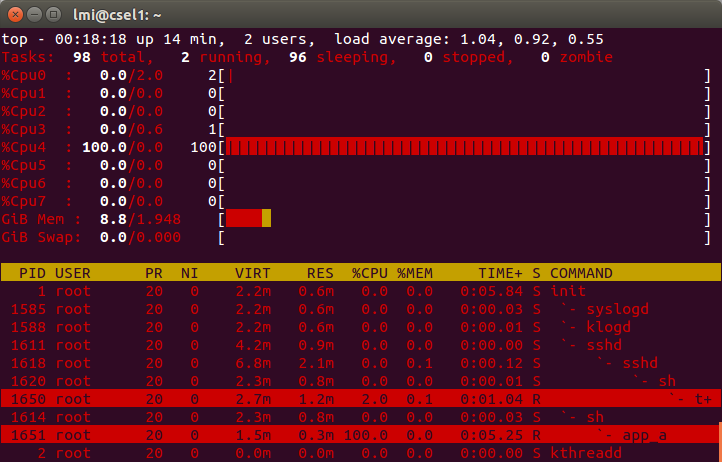
\includegraphics[width=14cm]{img/top2.png}
		\caption{Occupation du cœur avant modifications}
		\label{top2}
	\end{center}
\end{figure}
L'image ci-dessous montre que notre application est meilleure, elle consomme moins de 3\% d'un cœur.
\begin{figure}[H]
	\begin{center}
		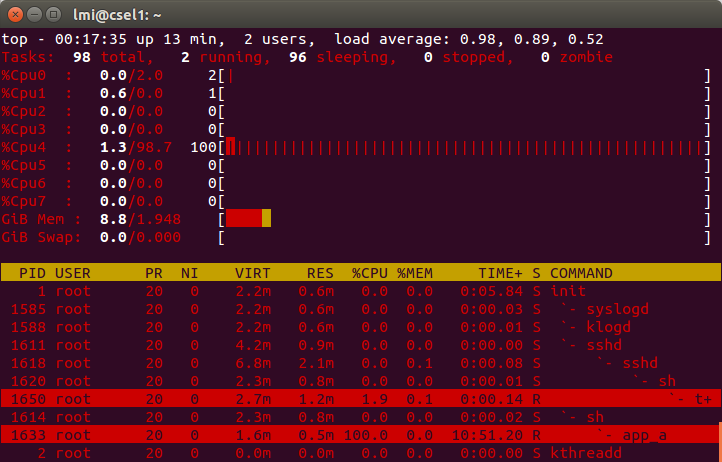
\includegraphics[width=14cm]{img/top1.png}
		\caption{Occupation du cœur après modifications}
		\label{top1}
	\end{center}
\end{figure}
\subsubsection{Amélioration possibles}
Les switch n'ont pas d'anti-rebond. Parfois, l'état du bouton du programme ne correspond pas à l'état physique du bouton. La conséquence est que le duty cylcle s'incrémente/décrémente alors qu'aucun bouton n'est appuyé. Il faudrait implémenter un anti-rebond software. Ce point n'a pas été réalisé, car ce n'était pas l'objectif du labo. Si le problème se présente, il suffit de relancer le programme.